%\documentclass[%
% aip,
% jmp,%
% amsmath,amssymb,
%%preprint,%
% reprint,%
%%author-year,%
%%author-numerical,%
%]{revtex4-1}
%%\documentclass[12pt]{article}
%\usepackage{amsmath, amssymb, graphicx}
%\usepackage[T1]{fontenc}
%\usepackage[latin9]{inputenc}
%\usepackage[margin=1in]{geometry} 
%\usepackage{url}
%\usepackage{amsthm,amsmath,amssymb}
%\usepackage{mathrsfs}
%\usepackage{makeidx}
%\usepackage{microtype}
%\usepackage{setspace}
%\usepackage{graphicx}
%\usepackage{ulem}
%\usepackage{url}
%\usepackage{enumerate}
%\usepackage{tikz}
%\usepackage{listings}
%\usepackage{thmtools}
%\usepackage{fancyhdr}
%\usepackage{float}
%\usepackage{tabularx}
%\usepackage{ragged2e}
%\usepackage{booktabs}
%\usepackage{caption}
%\usepackage{subcaption}
%\usepackage{mathtools}
%\usepackage{undertilde}
%%\usepackage[nottoc]{tocbibind}
%
%%\setlength{\textwidth}{6in}
%
%\author{Amal Agarwal}
%\title{Comparing Likelihood Free Algorithms for Matrix Normal Distribution via Gaussian Copula}
%\date{\today}
%\begin{document}
%\maketitle


% ****** Start of file aipsamp.tex ******
%
%   This file is part of the AIP files in the AIP distribution for REVTeX 4.
%   Version 4.1 of REVTeX, October 2009
%
%   Copyright (c) 2009 American Institute of Physics.
%
%   See the AIP README file for restrictions and more information.
%
% TeX'ing this file requires that you have AMS-LaTeX 2.0 installed
% as well as the rest of the prerequisites for REVTeX 4.1
%
% It also requires running BibTeX. The commands are as follows:
%
%  1)  latex  aipsamp
%  2)  bibtex aipsamp
%  3)  latex  aipsamp
%  4)  latex  aipsamp
%
% Use this file as a source of example code for your aip document.
% Use the file aiptemplate.tex as a template for your document.
%%%%%%%%%%%%%%%%%%%%%%%%%%%%%%%%%%%%%%%%%
% Journal Article
% LaTeX Template
% Version 1.3 (9/9/13)
%
% This template has been downloaded from:
% http://www.LaTeXTemplates.com
%
% Original author:
% Frits Wenneker (http://www.howtotex.com)
%
% License:
% CC BY-NC-SA 3.0 (http://creativecommons.org/licenses/by-nc-sa/3.0/)
%
%%%%%%%%%%%%%%%%%%%%%%%%%%%%%%%%%%%%%%%%%

%----------------------------------------------------------------------------------------
%	PACKAGES AND OTHER DOCUMENT CONFIGURATIONS
%----------------------------------------------------------------------------------------

\documentclass[twoside]{article}

%\usepackage[sc]{mathpazo} % Use the Palatino font
\usepackage[T1]{fontenc} % Use 8-bit encoding that has 256 glyphs
\linespread{1.05} % Line spacing - Palatino needs more space between lines
\usepackage{microtype} % Slightly tweak font spacing for aesthetics

\usepackage[hmarginratio=1:1,top=32mm,columnsep=20pt]{geometry} % Document margins
\usepackage{multicol} % Used for the two-column layout of the document
\usepackage[hang, small,labelfont=bf,up,textfont=it,up]{caption} % Custom captions under/above floats in tables or figures
\usepackage{booktabs} % Horizontal rules in tables
\usepackage{float} % Required for tables and figures in the multi-column environment - they need to be placed in specific locations with the [H] (e.g. \begin{table}[H])
\usepackage{hyperref} % For hyperlinks in the PDF

\usepackage{lettrine} % The lettrine is the first enlarged letter at the beginning of the text
\usepackage{paralist} % Used for the compactitem environment which makes bullet points with less space between them

\usepackage{abstract} % Allows abstract customization
\renewcommand{\abstractnamefont}{\normalfont\bfseries} % Set the "Abstract" text to bold
\renewcommand{\abstracttextfont}{\normalfont\small\itshape} % Set the abstract itself to small italic text

\usepackage{titlesec} % Allows customization of titles
%\renewcommand\thesection{\Roman{section}} % Roman numerals for the sections
%\renewcommand\thesubsection{\Roman{subsection}} % Roman numerals for subsections
\titleformat{\section}[block]{\large\scshape\centering}{\thesection.}{1em}{} % Change the look of the section titles
\titleformat{\subsection}[block]{\large}{\thesubsection.}{1em}{} % Change the look of the section titles

\usepackage{fancyhdr} % Headers and footers
\pagestyle{fancy} % All pages have headers and footers
\fancyhead{} % Blank out the default header
\fancyfoot{} % Blank out the default footer
\fancyhead[C]{LF-MCMC $\bullet$ Gaussian Copula $\bullet$ Matrix Normal $\bullet$ December 2015} % Custom header text
\fancyfoot[RO,LE]{\thepage} % Custom footer text
\usepackage{amsmath, amssymb, graphicx}
\usepackage[T1]{fontenc}
\usepackage[latin9]{inputenc}
%\usepackage[margin=1in]{geometry} 
\usepackage{url}
\usepackage{amsthm,amsmath,amssymb}
\usepackage{mathrsfs}
\usepackage{makeidx}
\usepackage{microtype}
\usepackage{setspace}
\usepackage{graphicx}
\usepackage{ulem}
\usepackage{url}
\usepackage{enumerate}
\usepackage{listings}
\usepackage{thmtools}
\usepackage{float}
\usepackage{tabularx}
\usepackage{ragged2e}
\usepackage{booktabs}
\usepackage{caption}
\usepackage{subcaption}
\usepackage{mathtools}
\usepackage{undertilde}
\usepackage{cite}
%\usepackage[nottoc]{tocbibind}

%\setlength{\textwidth}{6in}
%----------------------------------------------------------------------------------------
%	TITLE SECTION
%----------------------------------------------------------------------------------------

\title{\vspace{-15mm}\fontsize{16pt}{10pt}\selectfont\textbf{Comparing Likelihood Free MCMC Algorithms for Matrix Normal Distribution via Gaussian Copula\\}\vspace{0.08in}\fontsize{12pt}{5pt}\selectfont Statistical Computing STAT 540: Project Report} % Article title
%\subtitle{Statistical Computing STAT 540- Project Report}

\author{
\large
\textsc{Amal Agarwal}\thanks{Graduate Student, Department of Statistics}\\[2mm] % Your name
\normalsize Pennsylvania State University \\ % Your institution
\normalsize \href{mailto:aua257@psu.edu}{aua257@psu.edu} % Your email address
\vspace{-5mm}
}
\date{}

%----------------------------------------------------------------------------------------

\begin{document}

\maketitle % Insert title

\thispagestyle{fancy} % All pages have headers and footers

%----------------------------------------------------------------------------------------
%	ABSTRACT
%----------------------------------------------------------------------------------------

\begin{abstract}
Likelihood Free MCMC algorithms play a key role in Bayesian inference for situations when likelihood model is either intractable or computationally expensive\cite{brooks2011handbook}. These methods suffer from curse of diensioanlity and in high dimensions a procedure to implement them via Gaussian copula was introduced\cite{li2015extending}.  In certain situations, Matrix Normal distribution can prove very useful to model high dimensional data\cite{yin2012model}. This project compares different variants of LF-MCMC algorithms for Matrix Normal distribution via Gaussian copula.
\end{abstract}

%----------------------------------------------------------------------------------------
%	ARTICLE CONTENTS
%----------------------------------------------------------------------------------------

\begin{multicols}{2} % Two-column layout throughout the main article text

\section{Introduction} 
\label{sec:introduction}
There are many situations where the likelihood function $\pi(\utilde{y}|\theta)$ is either unavailable or computationally expensive. Common examples come from stochastic processes, particularly time series models. This poses challenge to obtain a significant effective sample size within reasonable amount of time since the chain runs very slowly. The classes of algorithms that have been developed to avoid evaluating likelihood function at each iteration of Metropolis Hastings (MH) algorithm are called Likelihood Free computations\cite{brooks2011handbook, beaumont2002approximate, marjoram2003markov, ratmann2009model, sisson2007sequential}.

Likelihood free methods have been gaining a lot of popularity in diverse applications where Bayesian inference via usual MH algorithm becomes computationally impractical\cite{brooks2011handbook}. Some of these applications include wireless communications engineering, quantile distributions, population genetics, protein networks, $\alpha$-stable models etc\cite{brooks2011handbook}.

The purpose of this project is three-fold. At first, we explore the broad topic of Likelihood free Markov Chain Monte Carlo (LF-MCMC) which comes under the umbrella of Approximate Bayesian Computations (ABC). We will review the basic idea and motivation behind using LF-MCMC algorithm over regular Metropolis Hastings (MH) algorithm\cite{brooks2011handbook}. We then briefly go over different variants of LF-MCMC listing out advantages and disadvantages of each algorithm. Secondly we go in deep to understand how LF-MCMC can be applied to high dimensional posteriors via Gaussian Copula. Lastly we will briefly go over Matrix Normal distribution and its advantages for modelling high dimensional data. We compare different variants of LF-MCMC for Matrix Normal likelihood model based on various criteria like effective sample size per second, total run time and mean square error for the estimated parameters\cite{li2015extending}.

\section{Likelihood Free MCMC}
\label{gmodels}

In its most trivial accept reject form, a LF algorithm consists of the following steps:
\begin{itemize}
\item Sample $\theta' \sim \pi(.)$ from the prior.
\item Generate dataset $\utilde{x}$ from the model $\pi(.|\theta')$.
\item Accept $\theta'$ if $\utilde{x}\approx \utilde{y}$, where $\utilde{y}$ is the observed dataset. 
\end{itemize}

The last step is crucial. If the simulated and observed datasets are similar in some manner, we regard $\theta'$ as a plausible candidate sample from out target posterior since there is a high chance this $\theta'$ could have generated the observed data from the given model. These steps form the basis of LF-MCMC algorithm and its variants to be described section 2.2. Note that here we have circumvented the problem of evaluation of likelihood function and replaced it with the problem of assessing if the simulated dataset is close to observed dataset in some manner.

To assess the closeness of two datasets, we usually use some kind of statistical distance metric like Euclidean, Mahalanobis, Minkowski etc. For continuous distributions the probability that the simulated dataset is equal to the observed dataset is exactly zero and so the acceptance rate of the above algorithm is also zero. To resolve this, we reduce the dimension of the dataset by using some sufficient statistic $T(.)$ for $\theta$ and assess if $T(\utilde{x})\approx T(\utilde{y})$. The idea is that there can be more than one simulated datasets which obey $T(\utilde{x})\approx T(\utilde{y})$, thus increasing aceptance probability.

\subsection{Theoretical background}
A natural question to ask is how the above formalism can be incorporated in MH algorithm and if so, why would it work. Recall that our target is $\pi(\theta|\utilde{y})$. Consider the following new augmented posterior target: \begin{equation}
\pi_{\text{LF}}(\theta,\utilde{x}|\utilde{y}) \propto \pi(\utilde{y}|\utilde{x},\theta)\pi(\utilde{x}|\theta)\pi(\theta)
\end{equation}
Here the auxilliary parameter $\utilde{x}$, is the simulated dataset from $\pi(.|\theta)$. The last two terms make up the posterior $\pi(\theta|\utilde{x})$ and the density $\pi(\utilde{y}|\utilde{x},\theta)$ puts more weight on this posterior in regions where $\utilde{x}$ and $\utilde{y}$ are similar i.e. $T(\utilde{x})\approx T(\utilde{y})$. For $\utilde{x}=\utilde{y}$, the density $\pi(\utilde{y}|\utilde{x},\theta)$ is assumed to be constant, thus returning back the target posterior exactly. Note that we are interested in the marginal posterior \begin{equation}
\label{eq2}
\pi_{\text{LF}}(\theta|\utilde{y}) \propto \pi(\theta) \int_{\mathcal{Y}}\pi(\utilde{y}|\utilde{x},\theta)\pi(\utilde{x}|\theta)d\utilde{x}
\end{equation} which acts as an approximation to $\pi(\theta|\utilde{y})$. We can simply discard the realizations of auxilliary data sets in order to perform the above integration numerically.

Now the augmented proposal directed towards an MCMC sampler for $\pi_{\text{LF}}(\theta,\utilde{x}|\utilde{y})$ can be factorized as 
\begin{equation}
q[(\theta,\utilde{x}),(\theta',\utilde{x'})]=q(\theta,\theta')\pi(\utilde{x}'|\theta')
\end{equation}
This means that given the current state $\theta$ we first sample $\theta'$ from the proposal $q(\theta,\theta')$ and then given this $\theta'$ we simulate a data set $\utilde{x}$ from our likelihood model. Using standard arguments of detailed balance and Harris ergodicity, we can show the stationarity of the augmented proposal. The probability of going from the current state $(\theta,\utilde{x})$ to the next state $(\theta',\utilde{x}')$ within the MH framework is just $\text{min}(1,\alpha[(\theta,\utilde{x}),(\theta',\utilde{x}')])$ where
\begin{align*}
\alpha[(\theta,\utilde{x}),(\theta',\utilde{x}')]=&\dfrac{\pi_{\text{LF}}(\theta',\utilde{x}'|\utilde{y})\hspace{0.05in}q[(\theta',\utilde{x}'),(\theta,\utilde{x})]}{\pi_{\text{LF}}(\theta,\utilde{x}|\utilde{y})\hspace{0.05in}q[(\theta,\utilde{x}),(\theta',\utilde{x}')]}\\
=&\dfrac{\pi(\utilde{y}|\utilde{x}',\theta')\pi(\utilde{x}'|\theta')\pi(\theta')}{\pi(\utilde{y}|\utilde{x},\theta)\pi(\utilde{x}|\theta)\pi(\theta)}\times\\
&\dfrac{q(\theta',\theta)\pi(\utilde{x}|\theta)}{q(\theta,\theta')\pi(\utilde{x}'|\theta')}\\=&\dfrac{\pi(\utilde{y}|\utilde{x}',\theta')\pi(\theta')q(\theta',\theta)}{\pi(\utilde{y}|\utilde{x},\theta)\pi(\theta)q(\theta,\theta')}
\end{align*}

This shows that the intractable likelihoods do not need to be evaluated in the acceptance probability calculation. The density function $\pi(\utilde{y}|\utilde{x},\theta)$ is usually approximated by kernel density estimation methods as 
\begin{equation}
\pi_{\epsilon}(\utilde{y}|\utilde{x},\theta) \varpropto \dfrac{1}{\epsilon}K\left(\dfrac{d(T(\utilde{y}),T(\utilde{x}))}{\epsilon}\right)
\end{equation}
Here $d(.)$ is some statistical distance metric, $K$ is some standard kernel density function like uniform, gaussian, epanechnikov etc. and $\epsilon$ is the scale parameter. 

If we take limit $\epsilon\rightarrow 0$ on the RHS, it would become a point mass on $T(\utilde{x})=T(\utilde{y})$, in which case the target posterior is exactly recovered. On the other hand if $\epsilon>0$ or if $T(.)$ is not sufficient statistics, then the LF approximation to $\pi(\theta|\utilde{y})$ is $\pi_{\text{LF}}(\theta|\utilde{y})$. Pseudocode for the corresponding LF-MCMC algorithm is given below:
\begin{enumerate}
\item Initialize $(\theta_0,\utilde{x}_0)$ and $\epsilon$. Set the iteration $t=0$.
\item At iteration t
\begin{enumerate}[(a)]
\item Generate $\theta'\sim q(\theta_t,\theta)$ from the proposal distribution of $\theta$.
\item Generate $\utilde{x}'\sim \pi(\utilde{x}|\theta')$ from the model given $\theta'$. 
\item With probability $\text{min}(1,\alpha[(\theta,\utilde{x}),(\theta',\utilde{x}')])$, set $(\theta_{t+1},\utilde{x}_{t+1})=(\theta',\utilde{x}')$, otherwise set $(\theta_{t+1},\utilde{x}_{t+1})=(\theta_{t},\utilde{x}_{t})$.
\item Set $t\leftarrow (t+1)$ and repeat step 2 until convergence.
\end{enumerate}
\end{enumerate}

\subsection{Variants of LF-MCMC algorithm}
\subsubsection{Error augmented sampler}
In all LF-MCMC algorithms, low values for the scale parameter $\epsilon$ results in high accuracy as suggested by taking the limit $\epsilon \rightarrow 0$. The disadvantage is slow mixing of chains through low acceptance rates. Increasing the $\epsilon$ value improves the chain mixing but accuracy is compromised. Optimizing over $\epsilon$ could be critical and the following error augmented sampler\cite{bortot2007inference} takes this into account by treating $\epsilon$ as a tempering parameter.
\begin{equation}
\pi_{\text{LF}}(\theta,\utilde{x},\epsilon|\utilde{y})\propto \pi_{\epsilon}(\utilde{y}|\utilde{x},\theta)\pi(\utilde{x}|\theta)\pi(\theta)\pi(\epsilon)
\end{equation}
The approximation to the target is then given by 
\begin{equation}
\pi_{\text{LF}}^{\mathcal{E}}(\theta|\utilde{y})\propto \int_{\mathcal{E}}\int_{\mathcal{Y}}\pi_{\text{LF}}(\theta,\utilde{x},\epsilon|\utilde{y})d\utilde{x}d\epsilon
\end{equation}
where $\epsilon \in \mathcal{E} \subseteq \mathcal{R}^+$

\subsubsection{Multiple augmented sampler}
To improve the sampler performance by reducing the variability in the acceptance probability, one approach is to use multiple augmented sampler\cite{andrieu2007expected}, where instead of simulating one dataset at each iterate, we simulate $S$ auxiliary datasets $\utilde{x}_{1:S}=(\utilde{x}^1,..., \utilde{x}^S)$ where $\utilde{x}^s \sim \pi(\utilde{x},\theta)$. The augmented target posterior becomes 
\begin{equation}
\pi_{\text{LF}}(\theta,\utilde{x}_{1:S}|\utilde{y}) \propto \dfrac{1}{S}\sum\limits_{s=1}^S\pi_{\epsilon}(\utilde{y}|\utilde{x}^{s},\theta)\prod\limits_{s=1}^S\pi(\utilde{x}^{s}|\theta)\pi(\theta)
\end{equation}
The approximation to the target is then given by 
\begin{equation}
\pi_{\text{LF}}^{S}(\theta|\utilde{y})\propto \int_{\mathcal{Y}^S}\pi_{\text{LF}}(\theta,\utilde{x}_{1:S}|\utilde{y})d\utilde{x}_{1:S}
\end{equation}

\subsubsection{Marginal space sampler}
Simulating $S$ datasets at each iterate similar to multiple augmented sampler, the integration in (\ref{eq2}), can be approximated by a Monte Carlo summation as 
\begin{equation}
\pi_{\text{LF}}(\theta|\utilde{y})\approx\dfrac{\pi(\theta)}{S}\sum\limits_{s=1}^S\pi_{\epsilon}(\utilde{y}|\utilde{x}^s,\theta)
\end{equation}
This permits to directly construct a LF-MCMC sampler targeting $\pi_{\text{LF}}(\theta|\utilde{y})$. With increase in $S$, the Monte Carlo approximation becomes more accurate. However the sampler performance is very poor in this case since it only approximates $\pi_{\text{LF}}(\theta|\utilde{y})$ which approximates $\pi(\theta|\utilde{y})$. An interesting thing to note is that the accepting probability of both Multiple augmented sampler and Marginal space sampler turns out to be exactly same. Thus both the samplers possess identical mixing and efficiency properties.

\section{LF-MCMC in high dimensions}
One of the primary restrictions to implement LF-MCMC algorithms is that they suffer from the curse of dimensionality \cite{blum2010non}. Kernel density estimation methods are reliable only in low dimensions. Also for parameter identifiability the dimension of $T(.)$ must be greater than or equal to dimension of $\utilde{\theta}$. These two constraints imply that the LF methods would perform poorly even with a moderate number of parameters. In specific situations like when the untractable likelihood is factorizable, this problem can be solved. However a general solution for constructing a LF approximation to the target in high dimensions is to construct a Gaussian copula that can approximate the dependence structure of $\pi(\utilde{\theta}|\utilde{y})$\cite{li2015extending}.

This approach relies on the fact that under standard regularity conditions, the posterior distribution  $\pi(\utilde{\theta}|\utilde{y})$ is asymptotically normal\cite{van2000asymptotic}. Now Meta Gaussian family of distributions has a peculiar property that the p-dimensional joint density can be reconstructed from all bivariate marginal densities. Thus using LF-MCMC methods, the bivariate densities can be estimated and then meta-Gaussian approximations of these densities can be combined together to form the neta-Gaussian approximation of the full posterior distribution. Let us first define a few things and set the notations:

Consider the random vector $\utilde{\theta}=(\theta_1,..., \theta_p)^T$ has continuous multivariate density $g(.)$. The marginal distribution functions and densities for $\theta_i$ are $G_i(.)$ and $g_i(.)$, $i=1,..., p$ respectively. The copula $C(\utilde{\theta})$ of is defined as the joint distribution of $\utilde{U}=(U_1,..., U_p)^T=(G_1(\theta_1),..., G_p(\theta_p))$ and contains the full dependence structure among all the components of $\utilde{\theta}$. Using Sklar's theorem theorem\cite{sklar1959fonctions}, we can write down $g(\utilde{\theta})=C(G_1(\theta_1),..., G_p(\theta_p))$. Now define $\utilde{\eta}=(\eta_1,..., \eta_p)^T$ with $\eta_i=\Phi^{-1}(G_i(\theta_i))$ for $i=1,..., p$ where $\Phi$ is the standard normal cumulative distribution function. If 
$\eta\sim N(0,\Lambda)$, then $C(\utilde{\theta})$ is called a Gaussian copula and $\utilde{\theta}$ has meta-Gaussian distribution function with density function:
\begin{equation}
\label{eq10}
g(\utilde{\theta})=\dfrac{1}{|\Lambda|^{1/2}}\text{exp}\left[\dfrac{1}{2}\eta^{T}(I-\Lambda^{-1})\eta\right]\prod\limits_{i=1}^{p}g_i(\theta_i)
\end{equation}
Also it is can be easily shown that multivariate normal family is embedded within the family of meta-Gaussian family\cite{li2015extending}. Using this fact and assuming the approximate normality of the target, we can implement the following algorithm to approximate $g(\utilde{\theta})$:

\begin{enumerate}
\item For each pair $(i,j)$ with $i=1,..., p-1$ and $j=i+1,..., p$,
\begin{enumerate}[(a)]
\item Identify the sufficient statistics $T_{(i,j)}$ for $(\theta_i,\theta_j)$.
\item Draw approximate samples $(\utilde{\theta}^{(1)},..., \utilde{\theta}^{(n)})$ using LF-MCMC algorithm (or one of its variant). Separate out the $(i,j)^{\text{th}}$ components as $(\theta_i^{(1)},\theta_j^{(1)}),..., (\theta_i^{(n)},\theta_j^{(n)})$.
\item Let $r_i^{(1)},..., r_i^{(n)}$ be the ranks of $\theta_i^{(1)},..., \theta_i^{(n)}$ and $q_j^{(1)},..., q_j^{(n)}$ be the ranks of $\theta_j^{(1)},..., \theta_j^{(n)}$. Put $\eta_i^{(l)}=\Phi^{-1}\left(\dfrac{r_i^{(l)}}{n+1}\right)$ and $\eta_j^{(l)}=\Phi^{-1}\left(\dfrac{q_j^{(l)}}{n+1}\right)$ for $l=1,..., n$.
\item Calculate the sample correlation $(\eta_i^{(1)}, \eta_j^{(1)}),..., (\eta_i^{(n)}, \eta_j^{(n)})$ and denote it as $\hat{\Lambda}_{i,j}=\hat{\Lambda}_{j,i}$.
\end{enumerate}
\item For $i=1,..., p$
\begin{enumerate}[(a)]
\item Identify the sufficient statistics $T_{(i)}$ for $(\theta_i)$.
\item Draw approximate samples $(\utilde{\theta}^{(1)},..., \utilde{\theta}^{(n')})$ using LF-MCMC algorithm (or one of tits variant). Separate the $i^{\text{th}}$ component as $\theta_i^{(1)},..., \theta_i^{(n')}$.
\item Approximate the marginal density $g_i(\theta_i)$ based on the above samples for the  $i^{\text{th}}$ component using density estimation methods. 
\end{enumerate}
\item Combine all the $\hat{\Lambda}_{\text{i,j}}'s$ from step 1 to form the $p$ dimensional correlation matrix $\hat{\Lambda}$. Using $\hat{\Lambda}$ and $\hat{g}_i(\theta_i)$, obtain an estimate of the approximation of the target using (\ref{eq10}). 
\end{enumerate}

The appoximation of the estimate of the target can be used in the Sampling Importance Resampling routine to generate samples from the this target. The steps are:
For $i=1,..., N$,
\begin{itemize}
\item Sample the vector from the importance function $\utilde{\theta}_i\sim f(\utilde{\theta})$.
\item Calculate the weights $w^{(i)}\propto \dfrac{g(\utilde{\theta}_i)}{f(\utilde{\theta}_i)}$
\item Calculate the normalized weights.
\item Re-sample $\utilde{\theta}_1,..., \utilde{\theta}_N$ according to the normalized weights. 
\end{itemize}

\section{Matrix Normal Distribution}
Undirected Gaussian graph models provide a powerful tool to model conditional independencies in high dimensional data\cite{yuan2007model}. In particular for a Gaussian Markov Random Field (GMRF)\cite{friedman2001elements, friedman2008sparse}, we are generally interested in estimating the concentration matrix $C=\Sigma^{-1}$ where $\Sigma$ is the corresponding variance-covariance matrix. This is usually aimed at exploiting the sparsity of the concentration matrix which is common in many situations. There have been many algorithms developed to deal with this problem. The famous Graphical Lasso algorithm\cite{friedman2008sparse} provides a sparse and shrinkage estimator. Other algorithms like BIGQUIC\cite{hsieh2013big} can solve for upto one million variables. 

One of the key assumptions in all these type of algorithms is that the samples are independent and identically distributed from a multivariate Gaussian distribution. However in certain applications like gene expression data, there is often a correlation between $p$ genes collected over $q$ different tissues from the same subject. To better understand this, consider $\mathbf{X}$ to be the $p\times q$ matrix of the expression data, where the $j^{\text{th}}$ column corresponds to the expression data of $p$ genes measured in the $j^{\text{th}}$ tissue, and the $i^{\text{th}}$ row corresponds to gene expressions of the $i^{\text{th}}$ gene over $q$ different tissues\cite{yin2012model}. Instead of assuming that the columns or rows are independent, we assume that the matrix variate random variable $\mathbf{X}$ follows a matrix normal distribution\cite{dawid1981some}, where both row and column precision matrices can be specified. These precision matrices of the matrix normal distribution provide the conditional independence structures of the row and column variables, where the non-zero off-diagonal elements of the precision matrices correspond to conditional dependencies among the elements in row or column of the matrix normal distribution \cite{yin2012model}.

For a $n\times p$ random matrix $\mathbf{X}$, the pdf of the Matrix Normal distribution $\mathcal{MN}_{n\times p}(\mathbf{M,U,V})$ is given as:
\begin{align}
\label{eq11}
\begin{split}
&p(\mathbf{X|M,U,V})\propto \dfrac{1}{|\mathbf{V}|^{n/2}|\mathbf{U}|^{p/2}}\times\\ &\exp\left(-\dfrac{1}{2}tr(\mathbf{V}^{-1}(\mathbf{X}-\mathbf{M})^T\mathbf{U}^{-1}(\mathbf{X}-\mathbf{M}))\right)
\end{split}
\end{align}
For a non-sparse setting and assuming $n>p$, the time compexity of evaluating this likelihood is $O(n^3)$. Also the number of parameters involved are again of the order of $O(n^3)$. Thus to do Bayesian inference even for small matrix sizes, it becomes imperative that we use LF-MCMC methods tailored for high dimensions like the one described in previous section.

\section{Simulation}
This project focusses on comparing different variants of LF-MCMC algorithm described in (2.2) for obtaining samples from the posterior comprising of parameters $(\mathbf{M,U,V})$ from the Matrix Normal distribution via Gaussian copula approach for high dimensions. Here our likelihood model is same as described in (\ref{eq11}) and priors over each element of $(\mathbf{M,U,V})$ are set as improper uniform. 

Firstly, with arbitrary parameter settings, observed data $\mathbf{Y}$ was simulated using (\ref{eq11}). This was done using the fact that $\mathbf{X}\sim \mathcal{MN}_{n\times p}(\mathbf{M,U,V})$ if and only if $\mathrm{vec}(\mathbf{X})\sim \mathcal{N}_{np}(\mathrm{vec}(\mathbf{M}),\mathbf{V}\otimes \mathbf{U})$ where $\otimes$  denotes the Kronecker product and $\mathrm {vec} (\mathbf {M} )$ denotes the vectorization of $\mathbf {M}$. Now given this observed data, the correlation matrix $\Lambda$ and the marginal densities $g_i(\theta_i)$, where $\theta_i$ are different elements of $\mathbf {M,U,V}$, were estimated using the the algortihm described in section 3. Three variants of LF-MCMC viz. Basic LFMCMC, Error augmented LF-MCMC and Multiple augmented MCMC were implemented in steps 1(b) and 2(b) of this algorithm. For each variant, three different choices of distance metrics viz. Euclidean, Minkowski and Mahalanobis and three different Kernel functions viz. Uniform, Gaussian and Epanechnikov were considered. Lastly, using the sampling impotance resampling procedure the samples from the actual target $\pi(\mathbf{M,U,V}|\mathbf{Y})$ were obtained. 

\section{Results and Conclusion}
The main evaluating criteria were chosen as Effective Sample Size per second (ESS/s) and Total Mean Square Error (TMSE) for the parameter estimates.

In one simulation, each chain over the pairs and individual parameter components was run $10$ times for $10,000$ iterates adaptively i.e. after each time, the starting value and the tuning parameter in the proposal were updated. The mean ESS/s and MSE for all the chains over different pairs was calculated. To account for the variability in the estimates of ESS/s in one simulation, 50 simulations were used to calculate the grand mean ESS/s. TMSE can be calculated by adding the mean squared errors for each element of the parameter matrices  $\mathbf{M},\mathbf{U}$ and $\mathbf{V}$.

It was found that the Euclidean distance metric and Uniform kernel density function performed best among all the variants. For these choices, the grand mean ESS/s varies with different matrix sizes as follows:

\begin{figure}[H]
  \centering
    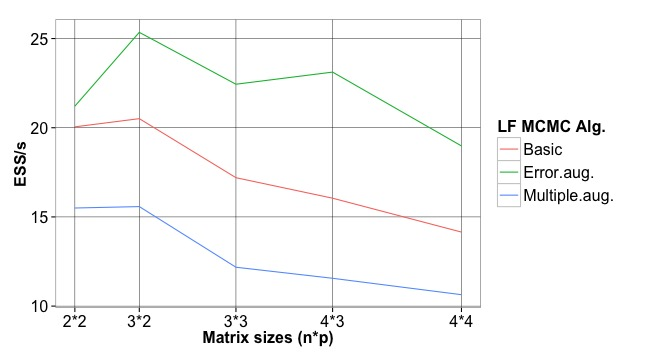
\includegraphics[width=0.35\textwidth]{plot1.jpeg}
    \caption{ESS/s vs. matrix sizes}
    \label{BN}
\end{figure}

The above plot clearly shows that error augmented sampler works better in terms of effective sample size per second. This can be attributed to the fact that while running the chains, $\epsilon$ is optimized for better chain mixing and accuracy. The variation of TMSE with increasing matrix sizes is given as:
\begin{figure}[H]
  \centering
    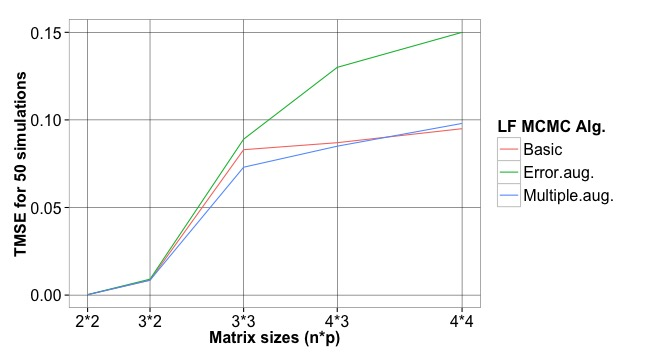
\includegraphics[width=0.35\textwidth]{plot2.jpeg}
    \caption{TMSE vs. matrix sizes}
    \label{BN}
\end{figure}

The above plot shows that the total mean square error for error augmented sampler is the highest. Running the chains longer solves this problem to some extent. But this clearly shows that the high effective sample size of this sampler is compromised by high TMSE. Also the multiple augmented sampler appears to be working better in terms of TMSE. This can be attributed to the fact that generating multiple datasets at each iterate help in reduction of the variance and thus faster convergence. The variation of mean total run time per simulation is given as follows:

\begin{figure}[H]
  \centering
    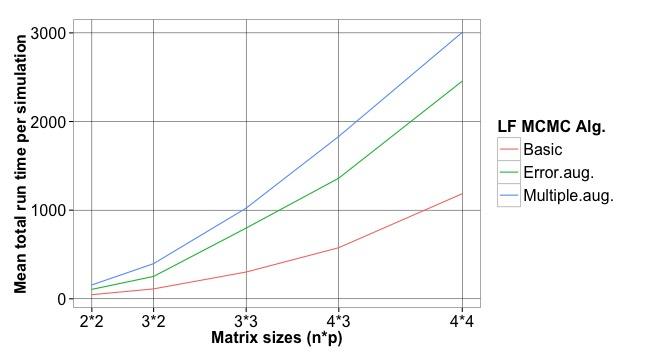
\includegraphics[width=0.40\textwidth]{plot3.jpeg}
    \caption{Mean total run time per simulation vs. matrix sizes}
    \label{BN}
\end{figure}

This plot clearly shows that multiple augmented sampler takes the most run time followed by error augmented sampler.

To assess the validity of the best performing algorithm, the diagnostic plots for the error augmented LF-MCMC sampler with Uniform kernel density function and Euclidean distance metric for one of the pairs, are given below:

\begin{figure}[H]
  \centering
    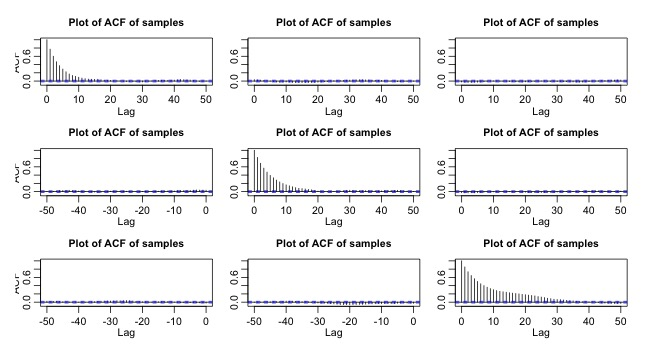
\includegraphics[width=0.30\textwidth]{plot8.jpeg}
    \caption{Plot of ACF of samples $(\theta_i,\theta_j,\epsilon)$}
    \label{BN}
\end{figure}

The above plot suggests a reasonable tuning parameter and good chain mixing.

\begin{figure}[H]
  \centering
    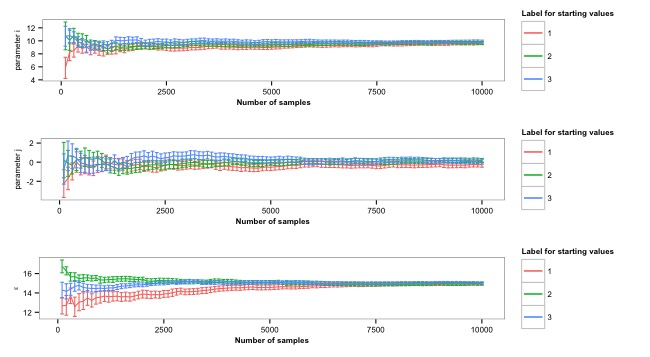
\includegraphics[width=0.30\textwidth]{plot4.jpeg}
    \caption{Plot of estimates vs. sample size with error bars for $(\theta_i,\theta_j,\epsilon)$}
    \label{BN}
\end{figure}

The above plot shows that for $(\theta_i,\theta_j,\epsilon)$ and for different starting values, the estimates converge to the same value.

\begin{figure}[H]
  \centering
    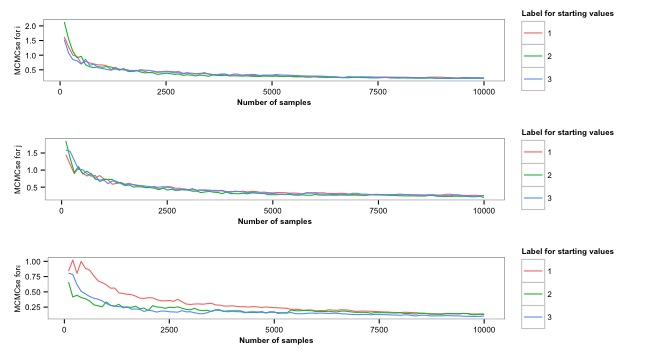
\includegraphics[width=0.30\textwidth]{plot5.jpeg}
    \caption{Plot of MCMC se vs. sample size for $(\theta_i,\theta_j,\epsilon)$}
    \label{BN}
\end{figure}

The above plot shows that for $(\theta_i,\theta_j,\epsilon)$ and for different starting values, MCMC standard errors converge to $0$. These two plots verifies the error augmented LF-MCMC sampler to some extent.

\begin{figure}[H]
  \centering
    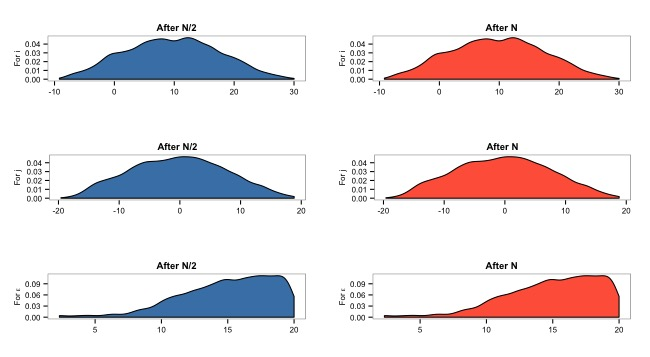
\includegraphics[width=0.30\textwidth]{plot6.jpeg}
    \caption{Plot of estimated density for $(\theta_i,\theta_j,\epsilon)$ after N/2 and N}
    \label{BN}
\end{figure}

\begin{figure}[H]
  \centering
    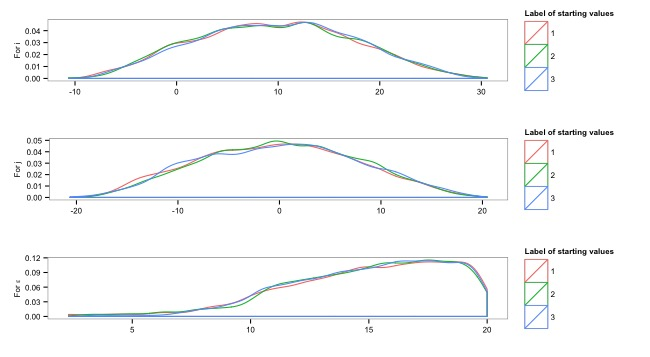
\includegraphics[width=0.30\textwidth]{plot7.jpeg}
    \caption{Plot of marginal density for $(\theta_i,\theta_j,\epsilon)$}
    \label{BN}
\end{figure}

From the above plots, the estimated densities after $n/2$ and after $n$ look reasonably identical for all the $3$ components. Also the estimated density for different starting values also overlap to a good extent. This further verifies the robustness and convergence of the algorithm.

\section{Discussion}
Although the basic sampler is suitable in terms of total run time, it is not recommended for smaller matrix sizes. However for larger matrix sizes it is the most optimum choice in terms of both ESS/s and TMSE. Error augmented samplers can be used in situations where precision is not required and we need fast mixing and high ESS/s. However with increasing matrix sizes the problem of TMSE appears to be increasing rapidly and longer chains may be required thus increasing the total run time. The multiple augmented sampler seems to be performing very bad in terms of ESS/s and total run time and therefore not recommended in general.
\section{Future work}
\begin{itemize}
\item It might be interesting to develop LF-MCMC algorithms that exploit the sparsity structure in the precision matrices $\mathbf{U}$ and $\mathbf{V}$
\item Tensor normal distributions of higher order can be studied under LF framework. 
\item I was not able to run another variant of LF-MCMC that aims for diagnosing mis-specification. If this works out, it might be helpful in model selection. 
\end{itemize}

\bibliography{bibfile}{}
\bibliographystyle{ieeetr} 

\end{multicols}
\end{document}
